% Practice Test 25 — Connecticut Edition
% Questions: 30 (21 MC + 9 SA)
% Generated by scripts/generate_practice_tests.py

\begin{practiceQuestion}{1-3-q26}{gmc}
\begin{questionText}
The graph below shows a proportional relationship. What is the constant of proportionality?

\begin{center}
\begin{tikzpicture}[scale=0.8]
  \draw[step=1,gray!20,thin] (0,0) grid (6,6);
  \draw[thick,->] (0,0) -- (6.5,0) node[right]{\small $x$};
  \draw[thick,->] (0,0) -- (0,6.5) node[above]{\small $y$};
  \foreach \x in {1,...,6} \draw (\x,0.07) -- (\x,-0.07) node[below]{\tiny \x};
  \foreach \y in {1,...,6} \draw (0.07,\y) -- (-0.07,\y) node[left]{\tiny \y};
  \draw[thick,funBlue] (0,0) -- (6,4);
  \fill[funBlue] (0,0) circle (2.5pt);
  \fill[funBlue] (3,2) circle (2.5pt) node[above left]{\small $(3, 2)$};
  \fill[funBlue] (6,4) circle (2.5pt) node[above left]{\small $(6, 4)$};
\end{tikzpicture}
\end{center}
\end{questionText}
\choiceA{$k = \frac{1}{2}$}
\choiceB{$k = \frac{2}{3}$}
\choiceC{$k = \frac{3}{2}$}
\choiceD{$k = 2$}
\correctAnswer{B}
\explanation{Use any labeled point: $k = \frac{2}{3}$ from $(3, 2)$. Check: $\frac{4}{6} = \frac{2}{3}$ \checkmark.}
\end{practiceQuestion}

\begin{practiceQuestion}{1-5-q26}{gmc}
\begin{questionText}
The graph below shows a proportional relationship between hours and miles traveled. What is the unit rate?

\begin{center}
\begin{tikzpicture}[scale=0.7]
  \draw[step=1,gray!20,thin] (0,0) grid (6,7);
  \draw[thick,->] (0,0) -- (6.5,0) node[right]{\small Hours};
  \draw[thick,->] (0,0) -- (0,7.5) node[above]{\small Miles};
  \foreach \x in {1,...,6} \draw (\x,0.07) -- (\x,-0.07) node[below]{\tiny \x};
  \foreach \y/\lab in {1/10,2/20,3/30,4/40,5/50,6/60,7/70}
    \draw (0.07,\y) -- (-0.07,\y) node[left]{\tiny \lab};
  \draw[thick,funBlue] (0,0) -- (6,5.4);
  \fill[funBlue] (0,0) circle (2.5pt);
  \fill[funBlue] (1,0.9) circle (2.5pt) node[above left]{\small $(1, 9)$};
  \fill[funBlue] (3,2.7) circle (2.5pt) node[above left]{\small $(3, 27)$};
  \fill[funBlue] (5,4.5) circle (2.5pt) node[above left]{\small $(5, 45)$};
\end{tikzpicture}
\end{center}
\end{questionText}
\choiceA{$3$ mph}
\choiceB{$9$ mph}
\choiceC{$27$ mph}
\choiceD{$45$ mph}
\correctAnswer{B}
\explanation{The point $(1, 9)$ directly gives the unit rate: $9$ miles per hour. Check: $\frac{27}{3} = 9$ and $\frac{45}{5} = 9$ \checkmark.}
\end{practiceQuestion}

\begin{practiceQuestion}{1-6-q02}{mc}
\begin{questionText}
A map scale says $2$ cm $= 15$ miles. Two cities are $7$ cm apart on the map. What is the actual distance?
\end{questionText}
\choiceA{$42.5$ miles}
\choiceB{$45$ miles}
\choiceC{$52.5$ miles}
\choiceD{$105$ miles}
\correctAnswer{C}
\explanation{Set up a proportion: $\frac{2}{15} = \frac{7}{d}$. Cross-multiply: $2d = 105$, so $d = 52.5$ miles.}
\end{practiceQuestion}

\begin{practiceQuestion}{2-1-q15}{mc}
\begin{questionText}
A library has $480$ books. If $35\%$ are fiction, how many fiction books does the library have?
\end{questionText}
\choiceA{$148$}
\choiceB{$160$}
\choiceC{$168$}
\choiceD{$172$}
\correctAnswer{C}
\explanation{$35\% = 0.35$. Multiply: $0.35 \times 480 = 168$ fiction books.}
\end{practiceQuestion}

\begin{practiceQuestion}{2-5-q18}{mc}
\begin{questionText}
Two friends split a $\$70$ dinner bill equally and each leave a $15\%$ tip on their share. How much does each person pay in total?
\end{questionText}
\choiceA{$\$35.00$}
\choiceB{$\$37.25$}
\choiceC{$\$40.25$}
\choiceD{$\$45.50$}
\correctAnswer{C}
\explanation{Each share: $70 \div 2 = \$35$. Tip: $35 \times 0.15 = \$5.25$. Total each: $35 + 5.25 = \$40.25$.}
\end{practiceQuestion}

\begin{practiceQuestion}{2-7-q30}{gsa}
\begin{questionText}
The bar graph shows the estimated and actual amounts of water (in liters) collected during an experiment over three days. On which day was the percent error the largest, and what was it?

\begin{center}
\begin{tikzpicture}[scale=0.5]
  \draw[thick,->] (0,0) -- (0,6.5) node[above]{\small Liters};
  \draw[thick,->] (0,0) -- (10.5,0);
  % Day 1: est 10, actual 8
  \fill[funBlue!60] (0.5,0) rectangle (1.5,5);
  \fill[funGreen!60] (1.5,0) rectangle (2.5,4);
  % Day 2: est 6, actual 5
  \fill[funBlue!60] (3.5,0) rectangle (4.5,3);
  \fill[funGreen!60] (4.5,0) rectangle (5.5,2.5);
  % Day 3: est 8, actual 10
  \fill[funBlue!60] (6.5,0) rectangle (7.5,4);
  \fill[funGreen!60] (7.5,0) rectangle (8.5,5);
  \node[below,font=\small] at (1.5,0) {Day 1};
  \node[below,font=\small] at (4.5,0) {Day 2};
  \node[below,font=\small] at (7.5,0) {Day 3};
  \foreach \y/\lab in {1/2,2/4,3/6,4/8,5/10,6/12} {
    \draw (-0.1,\y) -- (0.1,\y) node[left,font=\small,xshift=-2pt] {\lab};
  }
  \node[above,font=\scriptsize,funBlue] at (1,5) {$10$};
  \node[above,font=\scriptsize,funGreen!80!black] at (2,4) {$8$};
  \node[above,font=\scriptsize,funBlue] at (4,3) {$6$};
  \node[above,font=\scriptsize,funGreen!80!black] at (5,2.5) {$5$};
  \node[above,font=\scriptsize,funBlue] at (7,4) {$8$};
  \node[above,font=\scriptsize,funGreen!80!black] at (8,5) {$10$};
  % Legend
  \fill[funBlue!60] (0.5,6.3) rectangle (1,6.7);
  \node[right,font=\scriptsize] at (1.1,6.5) {Estimated};
  \fill[funGreen!60] (3.5,6.3) rectangle (4,6.7);
  \node[right,font=\scriptsize] at (4.1,6.5) {Actual};
\end{tikzpicture}
\end{center}
\end{questionText}
\correctAnswer{Day 1 with $25\%$ error}
\explanation{Day 1: $|10-8|/8 = 25\%$. Day 2: $|6-5|/5 = 20\%$. Day 3: $|8-10|/10 = 20\%$. Day 1 has the largest percent error at $25\%$.}
\end{practiceQuestion}

\begin{practiceQuestion}{3-1-q20}{sa}
\begin{questionText}
Find $|{-23}|$.
\end{questionText}
\correctAnswer{$23$}
\explanation{The absolute value of $-23$ is its distance from $0$, which is $23$.}
\end{practiceQuestion}

\begin{practiceQuestion}{3-2-q22}{sa}
\begin{questionText}
What is $(-18) + 18$?
\end{questionText}
\correctAnswer{$0$}
\explanation{$-18$ and $18$ are additive inverses (opposites). Their sum is always $0$.}
\end{practiceQuestion}

\begin{practiceQuestion}{4-1-q04}{mc}
\begin{questionText}
Evaluate $2a + 7$ when $a = -3$.
\end{questionText}
\choiceA{$13$}
\choiceB{$1$}
\choiceC{$-13$}
\choiceD{$-1$}
\correctAnswer{B}
\explanation{Substitute: $2(-3) + 7 = -6 + 7 = 1$.}
\end{practiceQuestion}

\begin{practiceQuestion}{4-2-q04}{mc}
\begin{questionText}
Simplify $3y + 8 - 5y - 2$.
\end{questionText}
\choiceA{$8y + 6$}
\choiceB{$-2y + 6$}
\choiceC{$2y - 6$}
\choiceD{$-2y + 10$}
\correctAnswer{B}
\explanation{Combine variable terms: $3y - 5y = -2y$. Combine constants: $8 - 2 = 6$. Result: $-2y + 6$.}
\end{practiceQuestion}

\begin{practiceQuestion}{5-2-q29}{gsa}
\begin{questionText}
The bar model shows an equation. Solve for $x$.

\begin{center}
\begin{tikzpicture}[scale=0.7]
  % Top bar: total
  \draw[thick,fill=funOrange!20] (0,1.5) rectangle (10,2.5);
  \node at (5,2) {$45$};
  % Bottom bar: split into parts
  \draw[thick,fill=funBlue!20] (0,0) rectangle (3,1);
  \node at (1.5,0.5) {$x$};
  \draw[thick,fill=funBlue!20] (3,0) rectangle (6,1);
  \node at (4.5,0.5) {$x$};
  \draw[thick,fill=funBlue!20] (6,0) rectangle (9,1);
  \node at (7.5,0.5) {$x$};
  \draw[thick,fill=funGreen!20] (9,0) rectangle (10,1);
  \node at (9.5,0.5) {$6$};
  % Brace
  \draw[decorate,decoration={brace,amplitude=5pt,mirror}] (0,-0.2) -- (10,-0.2);
\end{tikzpicture}
\end{center}
\end{questionText}
\correctAnswer{$x = 13$}
\explanation{The model shows $3x + 6 = 45$. Subtract $6$: $3x = 39$. Divide by $3$: $x = 13$.}
\end{practiceQuestion}

\begin{practiceQuestion}{5-3-q14}{mc}
\begin{questionText}
Solve $2(4x - 3) = 26$.
\end{questionText}
\choiceA{$x = 3$}
\choiceB{$x = 4$}
\choiceC{$x = 2$}
\choiceD{$x = 5$}
\correctAnswer{B}
\explanation{Distribute: $8x - 6 = 26$. Add $6$: $8x = 32$. Divide by $8$: $x = 4$. Check: $2(4 \cdot 4 - 3) = 2(13) = 26$ \checkmark.}
\end{practiceQuestion}

\begin{practiceQuestion}{5-4-q29}{gsa}
\begin{questionText}
The bar graph shows how much three students earned. Together they earned a total of $\$31.50$. Student C earned $\dfrac{1}{2}$ as much as Student A. Find how much Student C earned.

\begin{center}
\begin{tikzpicture}[scale=0.5]
  \draw[thick,->] (0,0) -- (0,11) node[above] {Dollars (\$)};
  \draw[thick,->] (0,0) -- (10,0);
  % Bars
  \draw[thick,fill=funBlue!40] (1,0) rectangle (3,8);
  \node[below] at (2,-0.3) {A};
  \node at (2,8.5) {$\$12$};
  \draw[thick,fill=funOrange!40] (4,0) rectangle (6,0);
  \node[below] at (5,-0.3) {B};
  \node at (5,1) {?};
  \draw[thick,fill=funGreen!40] (7,0) rectangle (9,0);
  \node[below] at (8,-0.3) {C};
  \node at (8,1) {?};
  % Y-axis labels
  \foreach \y in {0,2,...,10} {
    \draw (-0.2,\y) -- (0,\y);
    \node[left] at (-0.3,\y) {$\y$};
  }
\end{tikzpicture}
\end{center}

Student A earned $\$12$, and Student C earned $\dfrac{1}{2}$ of Student A's earnings.
\end{questionText}
\correctAnswer{$\$6$}
\explanation{Student C $= \frac{1}{2} \times 12 = \$6$. Check: Student B $= 31.50 - 12 - 6 = \$13.50$. Total: $12 + 13.50 + 6 = 31.50$ \checkmark.}
\end{practiceQuestion}

\begin{practiceQuestion}{5-5-q18}{mc}
\begin{questionText}
Solve $-x + 9 \leq 15$.
\end{questionText}
\choiceA{$x \leq -6$}
\choiceB{$x \geq 6$}
\choiceC{$x \geq -6$}
\choiceD{$x \leq 6$}
\correctAnswer{C}
\explanation{Subtract $9$: $-x \leq 6$. Multiply by $-1$ and flip: $x \geq -6$.}
\end{practiceQuestion}

\begin{practiceQuestion}{5-6-q18}{mc}
\begin{questionText}
Solve $6 - 2x \leq -4$ and describe the graph.
\end{questionText}
\choiceA{Closed circle at $5$, shade right}
\choiceB{Open circle at $5$, shade right}
\choiceC{Closed circle at $5$, shade left}
\choiceD{Closed circle at $-5$, shade right}
\correctAnswer{A}
\explanation{Subtract $6$: $-2x \leq -10$. Divide by $-2$ and flip: $x \geq 5$. Closed circle at $5$, shade right.}
\end{practiceQuestion}

\begin{practiceQuestion}{6-2-q19}{sa}
\begin{questionText}
A drawing uses $1$ cm $= 12$ m. You redraw at $1$ cm $= 4$ m. A hallway is $5$ cm on the original. How long is it on the new drawing?
\end{questionText}
\correctAnswer{$15$ cm}
\explanation{Scale ratio: $\frac{12}{4} = 3$. New length: $5 \times 3 = 15$ cm.}
\end{practiceQuestion}

\begin{practiceQuestion}{6-3-q13}{mc}
\begin{questionText}
A circle with radius $5$ cm is described as a condition. How many circles satisfy this condition?
\end{questionText}
\choiceA{None}
\choiceB{Exactly one}
\choiceC{More than one (different positions)}
\choiceD{It depends on the center location}
\correctAnswer{B}
\explanation{All circles with radius $5$ cm are congruent — they have the same shape and size. In terms of the figure itself (ignoring position), there is exactly one such circle.}
\end{practiceQuestion}

\begin{practiceQuestion}{6-4-q29}{gsa}
\begin{questionText}
Look at the triangle below. Two sides and the included angle are given. What is the condition type, and is the triangle unique?

\begin{center}
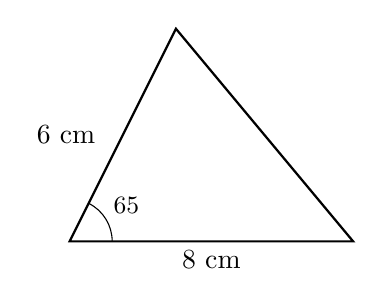
\begin{tikzpicture}[scale=0.9]
  \draw[thick] (0,0) -- (4,0) -- (1.5,3) -- cycle;
  \node[below] at (2,0) {$8$ cm};
  \node[left] at (0.5,1.5) {$6$ cm};
  \draw (0.6,0) arc[start angle=0,end angle=63,radius=0.6];
  \node at (0.8,0.5) {\small $65°$};
\end{tikzpicture}
\end{center}
\end{questionText}
\correctAnswer{SAS; yes, the triangle is unique}
\explanation{Two sides ($8$ cm and $6$ cm) and the included angle ($65°$) give the SAS condition. SAS always produces exactly one unique triangle.}
\end{practiceQuestion}

\begin{practiceQuestion}{6-5-q10}{mc}
\begin{questionText}
A cube can be sliced to produce a hexagonal cross-section. How?
\end{questionText}
\choiceA{By cutting parallel to the base}
\choiceB{By cutting diagonally through all six faces}
\choiceC{By cutting vertically through the center}
\choiceD{It is impossible to get a hexagon from a cube}
\correctAnswer{B}
\explanation{A diagonal plane that passes through all six faces of a cube creates a regular hexagonal cross-section.}
\end{practiceQuestion}

\begin{practiceQuestion}{7-3-q05}{mc}
\begin{questionText}
A pizza has a radius of $7$ inches. What is the area of the pizza? Use $\pi \approx \frac{22}{7}$.
\end{questionText}
\choiceA{$44$ in$^2$}
\choiceB{$154$ in$^2$}
\choiceC{$308$ in$^2$}
\choiceD{$22$ in$^2$}
\correctAnswer{B}
\explanation{$A = \pi r^2 = \frac{22}{7} \times 49 = 154$ in$^2$.}
\end{practiceQuestion}

\begin{practiceQuestion}{7-4-q01}{mc}
\begin{questionText}
A composite shape is made of a rectangle that is $10$ cm by $4$ cm and a triangle with base $10$ cm and height $3$ cm attached to one side. What is the total area?
\end{questionText}
\choiceA{$40$ cm$^2$}
\choiceB{$55$ cm$^2$}
\choiceC{$70$ cm$^2$}
\choiceD{$120$ cm$^2$}
\correctAnswer{B}
\explanation{Rectangle: $10 \times 4 = 40$ cm$^2$. Triangle: $\frac{1}{2} \times 10 \times 3 = 15$ cm$^2$. Total: $40 + 15 = 55$ cm$^2$.}
\end{practiceQuestion}

\begin{practiceQuestion}{7-5-q11}{mc}
\begin{questionText}
A cereal box is $30$ cm tall, $20$ cm wide, and $6$ cm deep. What is its surface area?
\end{questionText}
\choiceA{$1{,}440$ cm$^2$}
\choiceB{$1{,}560$ cm$^2$}
\choiceC{$1{,}800$ cm$^2$}
\choiceD{$3{,}600$ cm$^2$}
\correctAnswer{C}
\explanation{$SA = 2(30 \times 20) + 2(30 \times 6) + 2(20 \times 6) = 1200 + 360 + 240 = 1{,}800$ cm$^2$.}
\end{practiceQuestion}

\begin{practiceQuestion}{7-6-q23}{sa}
\begin{questionText}
A rectangular prism has a volume of $360$ cm$^3$. Its length is $12$ cm and its height is $5$ cm. What is its width?
\end{questionText}
\correctAnswer{$6$ cm}
\explanation{$360 = 12 \times w \times 5 = 60w$. $w = 360 \div 60 = 6$ cm.}
\end{practiceQuestion}

\begin{practiceQuestion}{8-1-q28}{gmc}
\begin{questionText}
The table below shows the results of two samples taken from a population of $1{,}000$ students.

\begin{center}
\begin{tabular}{|l|c|c|}
\hline
 & \textbf{Sample 1 (50 students)} & \textbf{Sample 2 (50 students)} \\
\hline
Prefer Math & $18$ & $22$ \\
\hline
Prefer Science & $14$ & $12$ \\
\hline
Prefer English & $10$ & $8$ \\
\hline
Prefer Art & $8$ & $8$ \\
\hline
\end{tabular}
\end{center}

Based on both samples, the best prediction for how many of the $1{,}000$ students prefer math is:
\end{questionText}
\choiceA{$180$}
\choiceB{$220$}
\choiceC{$400$}
\choiceD{$360$}
\correctAnswer{C}
\explanation{Average the two samples: $\frac{18+22}{2} = 20$ out of $50 = 40\%$. Then $40\%$ of $1{,}000 = 400$.}
\end{practiceQuestion}

\begin{practiceQuestion}{8-3-q16}{mc}
\begin{questionText}
Two histograms show that Group A's data is skewed left and Group B's data is symmetric. Which measure of center is most appropriate to compare them?
\end{questionText}
\choiceA{Mean for both}
\choiceB{Median for both}
\choiceC{Mode for both}
\choiceD{Range for both}
\correctAnswer{B}
\explanation{The median is less affected by skew than the mean, so it is the best measure to compare a skewed and a symmetric distribution.}
\end{practiceQuestion}

\begin{practiceQuestion}{8-4-q23}{sa}
\begin{questionText}
Data: $100, 200, 300, 400, 500$. Find the median and the IQR.
\end{questionText}
\correctAnswer{Median $= 300$; IQR $= 200$}
\explanation{Median (3rd value) $= 300$. $Q_1 = 200$, $Q_3 = 400$. IQR $= 400 - 200 = 200$.}
\end{practiceQuestion}

\begin{practiceQuestion}{9-1-q02}{mc}
\begin{questionText}
What does a probability of $1$ mean?
\end{questionText}
\choiceA{The event is impossible}
\choiceB{The event is unlikely}
\choiceC{The event has a $50\%$ chance}
\choiceD{The event is certain to happen}
\correctAnswer{D}
\explanation{A probability of $1$ means the event will definitely happen — it is certain.}
\end{practiceQuestion}

\begin{practiceQuestion}{9-4-q26}{gmc}
\begin{questionText}
Look at the spinner below. Which probability model correctly represents this spinner?

\begin{center}
\begin{tikzpicture}[scale=1.2]
  \fill[funRed!50] (0,0) -- (0:1.5) arc (0:180:1.5) -- cycle;
  \fill[funBlue!50] (0,0) -- (180:1.5) arc (180:270:1.5) -- cycle;
  \fill[funGreen!50] (0,0) -- (270:1.5) arc (270:360:1.5) -- cycle;
  \draw[thick] (0,0) circle (1.5);
  \draw[thick] (0,0) -- (0:1.5);
  \draw[thick] (0,0) -- (180:1.5);
  \draw[thick] (0,0) -- (270:1.5);
  \node at (90:0.8) {\textbf{Red}};
  \node at (225:0.8) {\textbf{Blue}};
  \node at (315:0.8) {\textbf{Green}};
\end{tikzpicture}
\end{center}
\end{questionText}
\choiceA{$P(\text{Red}) = \frac{1}{3}$, $P(\text{Blue}) = \frac{1}{3}$, $P(\text{Green}) = \frac{1}{3}$}
\choiceB{$P(\text{Red}) = \frac{1}{2}$, $P(\text{Blue}) = \frac{1}{4}$, $P(\text{Green}) = \frac{1}{4}$}
\choiceC{$P(\text{Red}) = \frac{1}{4}$, $P(\text{Blue}) = \frac{1}{4}$, $P(\text{Green}) = \frac{1}{2}$}
\choiceD{$P(\text{Red}) = \frac{1}{2}$, $P(\text{Blue}) = \frac{1}{2}$, $P(\text{Green}) = 0$}
\correctAnswer{B}
\explanation{Red covers half the spinner ($180\degree$), while Blue and Green each cover a quarter ($90\degree$ each). This is a non-uniform model.}
\end{practiceQuestion}

\begin{practiceQuestion}{9-6-q15}{mc}
\begin{questionText}
Two dice are rolled. What is the probability that the product (not the sum) of the two numbers is $12$?
\end{questionText}
\choiceA{$\frac{2}{36}$}
\choiceB{$\frac{4}{36}$}
\choiceC{$\frac{3}{36}$}
\choiceD{$\frac{6}{36}$}
\correctAnswer{B}
\explanation{Pairs with product $12$: $(2,6), (6,2), (3,4), (4,3)$ — that is $4$ out of $36$. $P = \frac{4}{36} = \frac{1}{9}$.}
\end{practiceQuestion}

\begin{practiceQuestion}{9-7-q10}{mc}
\begin{questionText}
A student simulates rolling two dice $36$ times to see how often the sum is $7$. They get a sum of $7$ a total of $8$ times. How does this compare to the expected number?
\end{questionText}
\choiceA{Expected: $6$; the simulation result ($8$) is slightly higher}
\choiceB{Expected: $6$; the simulation result ($8$) is much higher}
\choiceC{Expected: $12$; the simulation result ($8$) is lower}
\choiceD{Expected: $7$; the simulation result ($8$) is exact}
\correctAnswer{A}
\explanation{$P(\text{sum} = 7) = \frac{6}{36} = \frac{1}{6}$. Expected: $36 \times \frac{1}{6} = 6$. The simulation gave $8$, slightly above expected.}
\end{practiceQuestion}
